\chapter{Anexo}
\label{anexo}

%\section{Estado del Arte}
%\label{anexo.estadodelarte}

%\subsection{Gestión de incidentes}
%\label{anexo.gestiondeincidentes}
%\subsubsection{Herramientas}
%\label{anexo.herramientas}
%\subsubsection{Que es RTIR}
RTIR es un sistema de manejo de incidentes diseñado para ser utilizado por los 
equipos de seguridad de sistemas. A sido creado en conjunto con equipos de CERT 
y CSIRT para manejar el creciente número de incidentes reportados.
Presenta la ventaja de ser opensource, contener una API completa y una comunidad 
de usuarios grande y experta. Además es simple de integrar con otras 
herramientas existentes. Está implementado por medio de módulos PERL y las 
herramientas que provee RT. Se puede pensar en RTIR como una extensión de RT 
para ser utilizada por CERT's y CSIRT's.

Existen algunas alternativas a RTIR como lo son AIRT (Application for Incident Response Teams) 
cuya última versión data de Julio de 2009. AIRT es una aplicación web 
desarrollada para los equipos de respuesta a incidentes. Busca proveer facilidad 
ante los reportes de incidentes de seguridad así como un seguimiento simple de 
estos. Este sistema no cuenta con una comunidad comparable a la de RTIR así como 
con documentación tan extensa como la de RTIR.

Otra de las opciones existentes es OTRS (Open Technology Real Services), así 
como los anteriores también es open soruce. Presenta las ventajas de tener una 
comunidad más numerosa que AIRT y que el código esta siendo desarrollado continuamente. 
Así como RTIR esta desarrollado por medio de Perl y permite conectarse a varias 
bases de datos. Presenta documentación extensa para implementadores.

%\subsection{Representación}
%\label{anexo.representacion}
%\subsubsection{Modelos de datos}
%\label{anexo.modelodedatos}
%Aca se podria poner algo de openIOC

%\subsubsection{IDMEF}

Intrusion Detection Message Exchange Format (IDMEF) fue especificado como un 
protocolo experimental que no especifica ningún estándar. El propósito de 
IDMEF es definir formatos de datos y procedimientos de intercambio para 
compartir información de interés con sistemas de detección de intrusos y 
sistemas de respuesta con los sistemas de administración que deben 
interactuar con estos. El RFC de IDMEF describe el modelo de datos para 
representar información tomada de los sistemas de intrusión. Se busca que dicho 
formato pueda ser utilizado por los Intrusion Detection Systems (IDSs) para 
reportar alertas sobre eventos que parezcan sospechosos.

Por medio de la firma digital de XML se busca proveer integridad, autenticidad de 
los mensajes y de los servicios. La responsabilidad para la integridad y 
autenticación de los mensajes es responsabilidad del protocolo de comunicación y 
no del formato de mensajes. La inclusión de firmas digitales en mensajes IDMEF 
debería ser realizada en casos en los que éstas deban ser archivadas para su uso 
posterior o cuando los mensajes IDMEF son intercambiados sobre protocolos poco 
seguros.

\paragraph{Modelo de datos de IDMEF}
El modelo de datos de IDMEF es una representación orientada a alertas enviadas a 
los administradores desde los sistemas de intrusión. El modelo de datos presenta 
varios problemas referentes a la representación de los datos:
\begin{itemize}
  \item Generalmente, la información de las alertas es heterogénea. Algunas 
  alertas son definidas con poca información, otras proveen información más 
  detallada. Ejemplos de alertas con poca información son aquellas que solo 
  presentan datos de origen, destino, nombre u hora, estos datos pueden set 
  extendidos por alertas detalladas en las cuales se presenta información de 
  usuarios, procesos o puertos de servicios. Es necesario que el modelo de datos 
  que represente dicha información sea flexible para adaptarse a las distintas 
  necesidades. Un modelo de datos orientado a objetos es extensible por medio de 
  agregación y sub clases, de esta forma una implementación que no entienda 
  estas extensiones podrá seguir entendiendo el subconjunto de información que 
  está definido en el modelo. Estas dos formas de extender el modelo permiten 
  que se mantenga su consistencia.
  \item Los IDSs son diferentes, algunos de estos detectan ataques analizando el 
  tráfico en la red, otros utilizando los logs de sistemas operativos o 
  aplicaciones que auditan información. Las alertas generadas para un mismo 
  ataque pero por medio de diferentes herramientas, no necesariamente contienen 
  los mismos datos. El modelo de datos define clases que soportan las 
  diferencias en las fuentes de los datos. En particular, las nociones de 
  fuente y objetivo para la alerta son representadas por una combinación de 
  nodo, procesos, servicio y clases de usuario.
  \item Dependiendo del tipo de red o sistema operativo utilizado, los 
  ataques serán observados y reportados de manera diferente lo cual lleva a que 
  el modelo de datos deba adaptarse a dichas diferencias.
  \item Los instrumentos comerciales persiguen objetivos diferentes. Por varias 
  razones, estos desean entregar más o menos información sobre ciertos tipos de 
  ataques. El modelo debe permitir la flexibilidad necesaria preservando su 
  integridad.
\end{itemize}

El diseño del modelo de datos busca proveer una representación estándar de las 
alertas de manera que la información no sea ambigua y que se describa la 
relación entre alertas simples y complejas.

El objetivo de dicho modelo es proveer una representación estándar de la 
información analizada por un sistema de intrusión cuando es detectado 
un evento inusual. Estas alertas pueden ser simples o complejas 
dependiendo de las capacidades de la herramienta que las creo.

Los nuevos objetos son introducidos para referenciar contenido adicional. Esto 
es importante debido a que la tarea de clasificar y nombrar vulnerabilidades es 
difícil y sumamente subjetiva. El modelo de datos no debe ser ambiguo, por lo 
que mientras que se permite que los análisis sean más o menos precisos 
entre ellos, no se debe permitir que estos produzcan información contradictoria  
en dos alertas que describen el mismo evento. De todas formas, siempre es 
posible insertar toda la información útil de un evento en campos de extensión 
de la alerta en lugar de en los campos a los que estos pertenecen, sin embargo, 
dichas prácticas reducen la interoperabilidad y deberían ser evitadas en lo 
posible.



%\subsubsection{IODEF}

\textit{Incident Object Description Exchange Format} (IODEF) define una representación de datos que provee un framework para el 
intercambio de información entre CSIRTs, dicho tipo de información de seguridad 
es comúnmente intercambiado entre este tipo de organizaciones. IODEF provee una 
representación en XML para transportar información de incidentes entre pares en 
distintos dominios administrativos pero que tienen las responsabilidades 
operacionales de remediar o analizar y establecer advertencias en un dominio 
definido. El modelo de datos provisto por IODEF codifica la información 
referente a hosts, redes y servicios corriendo en estos sistemas; metodología 
de ataques y evidencia forense asociada; impacto de la actividad realizada y
aproximaciones a los trabajos realizados.\\

IODEF debería ser compatible con IDMEF y tener la capacidad de incluir mensajes 
IDMEF. Los actores principales en IODEF son los CSIRTs y no los IDSs como ocurre 
en IDMEF. Se puede ver a IODEF como una interfaz orientada a ser utilizada por 
personas, por ello un mensaje IODEF es parseable por una máquina y a su vez 
leíble por humanos. Los objetos IODEF tienen un tiempo de vida mayor a IDMEF, 
en éste último los mensajes son utilizados una sola vez. Los mensajes IODEF consideran 
información referente al manejo de incidentes, almacenamiento de dicha 
información o estadísticas y análisis.\\

El objetivo primordial de IODEF es mejorar las capacidades operacionales de los 
CSIRTs. La adopción por parte de la comunidad provee una habilidad mejorada para 
resolver los incidentes y transmitir información de contexto simplificando la 
colaboración e intercambio de datos.
El formato estructurado provisto por IODEF permite:
\begin{itemize}
  \item Incrementar la automatización en el procesamiento de los datos.
  \item Bajar el esfuerzo necesario para normalizar datos similares de 
  diferentes fuentes.
  \item Un formato común con el cual construir herramientas interoperables para 
  el manejo de incidentes y análisis subsecuente, específicamente cuando 
  los datos provienen de dominios distintos.
\end{itemize}

La coordinación entre CSIRTs no es un problema estrictamente técnico. La 
confianza, los procedimientos y las leyes son consideraciones que pueden impedir 
que las organizaciones intercambien información. IODEF no busca evadir dichas 
consideraciones, sin embargo, las implementaciones operacionales de IODEF deben 
considerar este contexto.

\paragraph{Modelo de datos de IODEF}\ \\

A la hora de diseñar IODEF se realizaron ciertas consideraciones de diseño:
\begin{itemize}
  \item El modelo de datos sirve como formato de transporte, lo que lleva a que 
  su representación específica no sea óptima para almacenamiento en disco, 
  ser archivado por plazos largos o procesamiento en memoria.
  \item Por medio de la implementación no se busca establecer un consenso 
  respecto a la definición de un incidente, en su lugar se trata de dar un 
  entendimiento amplio que sea lo suficientemente flexible para abarcar la 
  mayoría de las operaciones.
  \item Describir un incidente para todas las definiciones requeriría un modelo 
  de datos extremadamente complejo. Por ello, IODEF solo busca dar un marco para 
  transmitir información de incidentes comúnmente intercambiada. Se asegura un 
  mecanismo que pueda ser extendido para soportar información de la 
  organización así como técnicas para referenciar información mantenida por 
  fuera del modelo de datos.
  \item El dominio de análisis de seguridad no está totalmente estandarizado y 
  debe basarse en descripciones textuales. IODEF busca conseguir un balance 
  entre el contenido libre y el procesamiento automático de la información de 
  incidentes.
  \item IODEF es una de las representaciones que han sido estandarizadas.
   El modelo de datos de IDMEF influenció el diseño de IODEF.

\end{itemize}

El modelo de datos de IODEF no introduce problemas de seguridad. Este solo 
define una representación simple para información de incidentes. Como los datos 
codificados por IODEF pueden ser considerados sensibles por las partes que los 
intercambian se deben tomar precauciones para asegurar la confidencialidad 
durante el intercambio y el subsecuente procesamiento. El primero debe ser 
resguardado por un formato de mensaje, pero luego se deben tener consideraciones 
de seguridad en el sistema que procesa los datos, los almacena y archiva la 
documentación y la información derivada de éstos.\\

El formato de mensajes subyacente y el protocolo utilizado para intercambiar 
datos provee una garantía de confidencialidad, integridad y autenticidad. El uso 
de protocolos de seguridad estandarizados es recomendado, por ejemplo 
IODEF/RID.

\paragraph{Trabajo de MILE}\ \\

\textit{Managed Incident Lightweight Exchange} (MILE) es un grupo de trabajo del IETF que 
enfoca sus esfuerzos en dos áreas. La primera es el formato de datos y 
extensiones para representar incidentes y datos de indicadores con IODEF. La segunda área 
es el protocolo RID.\\

Respecto a IODEF se busca revisar el RFC para incorporar mejoras y extensiones 
basándose en la experiencia que ha sido obtenida de su utilización. Se busca poder extender IODEF para 
soportar extensiones específicas necesarias por la industria y permitir utilizar 
contenido específico. Además MILE busca proveer guías en la implementación y uso 
de IODEF para ayudar a los implementadores en el desarrollo de sistemas.\\

Respecto a RID se busca definir una aproximación orientada a los recursos que 
permita a los CSIRTs ser más dinámicos y ágiles a la hora de colaborar. También 
se busca proveer guías en la implementación y uso de RID. RID podría requerir 
modificaciones para agregar información de políticas u otros cambios. Con el 
incremento en la cantidad de implementaciones RID, podría ser necesaria una 
revisión de su RFC.



%\input{./anexo/OPENIOC}
%\subsubsection{STIX}

Structured Threat Information eXpression (STIX) es un lenguaje para la especificación, captura, representación y 
comunicación de información de seguridad. Lo realiza de manera 
estructurada para soporteortar un mejor manejo de la información así como para 
permitir procesos automatizados.\\

Se busca que la información sea representada de forma estructurada, a su vez 
esta debe ser expresiva, flexible, extensible, automatizable y legible. Esto se 
presenta como un desafío ya que la información intercambiada debe ser 
estructurada para que pueda ser parseada por una máquina pero no se debe perder 
la posibilidad de que un analista la pueda leer y entender. Que sea entendible 
por una persona es necesario para que no se pierda el juicio y control que esta 
pueda tener.\\

Al convertirse STIX en un estándar para la comunidad se obtendrá información de 
mejor calidad la que será mejor aprovechada y de la cual no se sabrá la fuente 
de los datos de antemano.

\paragraph{Aproximaciones de la actualidad}\ \\

La información que se intercambia y utiliza actualmente es atómica, inconsistente 
y muy limitada en sofisticación y expresividad. Además, el uso de estructuras 
estandarizadas se enfoca en una porción del problema y la integración no se 
realiza de forma adecuada entre si o carece de la flexibilidad para hacerlo. 
Generalmente, las actividades de intercambio de indicadores son entre humanos, 
siendo los indicadores desestructurados o semi-estructurados e intercambiados 
por medio de portales web o encriptados y enviados vía email. Recientemente se 
ha visto el surgimiento de transferencias entre máquinas, éstas intercambian 
conjuntos de indicadores simples de modelos de ataques bien conocidos.\\

A diferencia de IODEF, STIX provee una lista de elementos para construir 
indicadores de compromiso y se integra con CAPEC, MAEC o CVE. Además posee 
soporte para tácticas, técnicas y procedimientos del adversario y tareas 
realizadas por la organización. IODEF fue pensado para compartir información de 
incidentes y no indicadores de compromiso. STIX permite el intercambio de 
indicadores referentes a amenazas así como información del contexto en el que 
éstas se dan. Juntos, permiten tener un conocimiento más rico de las 
intenciones, capacidades, motivaciones y actividades de un adversario y de esta 
forma defenderse de él.\\

STIX busca extender los indicadores para permitir el manejo e intercambio de 
estos de forma más expresiva y con un espectro más amplio de información.\\

Actualmente, el intercambio y manejo de información automática es visto 
típicamente en líneas de productos, servicios ofrecidos o soluciones específicas 
de una comunidad. STIX busca permitir el intercambio de información de forma 
comprensiva, rica, de alta fidelidad entre organizaciones, comunidades, 
productos y servicios ofrecidos.\\

STIX provee una arquitectura unificada con un conjunto amplio de información 
para permitir una solución práctica que permita la implementación de distintos 
casos de uso. El conjunto de información incluye:
\begin{itemize}
  \item Cyber Observables
  \item Indicadores
  \item Incidentes
  \item Tácticas, técnicas y procedimientos de los adversarios
  \item Objetivos de exploits
  \item Cursos de acción
  \item Campañas de ataques
  \item Actores de ataques
\end{itemize}


\paragraph{Casos de uso}\ \\

El lenguaje STIX ha sido desarrollado para soportar varios casos de uso involucrados en el 
manejo de amenazas de seguridad. A continuación se dan descripciones de esos 
casos de uso.
\begin{itemize}
  \item \underline{Análisis de Cyber Amenazas}: Un analista de seguridad estudia información 
  estructurada y no estructurada referente a actividades de una amenaza 
  procedentes de varias fuentes. El analista busca entender la naturaleza de las 
  amenazas más relevantes, identificarlas, y representarlas para poder expresar 
  y actualizar el conocimiento relevante de la amenaza. La información de la 
  amenaza incluye acciones realizadas, comportamientos, capacidades, quienes lo 
  realizaron, etc. De este conocimiento y representación el analista puede 
  especificar patrones de la amenaza, sugerir acciones a ser realizadas para 
  responder a sus actividades y/o compartir información con socios de su 
  confianza.
  \item \underline{Especificar patrones de amenazas}: Un analista especifica patrones para 
  representar las características de amenazas junto con su contexto y metadatos 
  para interpretar, manejar y aplicar el patrón y sus resultados. Esto puede ser 
  realizado manualmente o con la asistencia de una herramienta automática.
  \item \underline{Manejo de las actividades de respuesta}: Los encargados de tomar decisiones y el personal de operaciones trabajan 
  en conjunto para prevenir o detectar actividades que presenten una amenaza y 
  responder a los incidentes detectados que sean realizados por dichas amenazas. 
  Las acciones preventivas pueden mitigar vulnerabilidades, debilidades o malas 
  configuraciones que sean objetivos de exploits. Luego de la detección e 
  investigación de incidentes específicos, acciones reactivas pueden ser 
  realizadas. Se pueden desprender tres sub-casos de uso de lo anterior.
  \begin{itemize}
    \item \underline{Prevención de amenazas}: Quienes deben tomar las decisiones evalúan 
    acciones preventivas para las amenazas relevantes que sean identificadas. Además deben crear acciones para mitigar dichas amenazas. El personal de 
    operaciones implementa las acciones seleccionadas por los tomadores de 
    decisión. Dichas medidas preventivas son obtenidas por medio de la 
    interpretación de los indicadores.
    \item \underline{Detección de amenazas}: El personal de operaciones aplica mecanismos 
    (automáticos y manuales) para monitorear y asistir las operaciones con la 
    finalidad de detectar la ocurrencia de amenazas específicas basándose en la 
    evidencia histórica, análisis del contexto actual e interpretación de los 
    indicadores que se presentan. Esta detección se realiza generalmente por 
    medio de patrones de indicadores.
    \item \underline{Respuesta a incidentes}: El personal de operaciones responde a amenazas 
    detectadas, investiga que ha ocurrido o está ocurriendo, trata de 
    identificar y representar la naturaleza de las amenazas y lleva a cabo 
    acciones para mitigar sus efectos, también puede aplicar acciones 
    preventivas. Una vez que los efectos son entendidos, el personal de 
    operaciones puede implementar acciones acordes para prevenir o llevar a cabo 
    tareas correctivas.
  \end{itemize} 
  \item \underline{Intercambio de información}: Los encargados de tomar las decisiones 
  establecen políticas respecto a que tipo de información será compartida, 
  además toma decisiones respecto a con quienes se comparte y como debería ser 
  manejada basándose en frameworks de confianza de forma de mantener niveles 
  adecuados de consistencia, contexto y control. Esta política es luego 
  implementada para compartir los indicadores de amenazas apropiados y otra 
  información de amenazas.
\end{itemize}

\paragraph{Principios de desarrollo de STIX}\ \\
En el enfoque dado a STIX se ha buscado implementar un conjunto de principios 
para su desarrollo con el consenso de la comunidad. Esos principios son los siguientes:
\begin{itemize}
  \item \underline{Expresividad}: Con el fin de soportar la diversidad de casos de uso relevantes, STIX apunta a 
proveer una cobertura expresiva en todos sus casos de uso específicos en lugar 
de dirigirse específicamente a alguno de ellos.
  \item \underline{Integración en lugar de duplicación}: Cuando STIX abarca conceptos de información estructurada para los cuales ya 
existen representaciones estandarizadas con el consenso adecuado y que se 
encuentran disponibles, se busca integrar estas representaciones a la 
arquitectura STIX en lugar de duplicar esta información innecesariamente.
\item \underline{Flexibilidad}: Con el fin de soportar un amplio rango de casos e información variable con 
varios niveles de fidelidad, se ha diseñado a STIX para ofrecer tanta flexibilidad 
como sea posible. STIX se adhiere a una política de permitir a los usuarios 
utilizar cualquier porción de representaciones estándar que sean relevantes para 
un contexto dado y evita elementos obligatorios siempre que sea posible.
\item \underline{Extensibilidad}: Con la finalidad de soportar un amplio rango de casos de uso con un potencial 
diferente de representación y para facilitar el perfeccionamiento 
impulsado por la comunidad, se ha diseñado STIX para construir mecanismos de 
extensión para usos específicos, para usos localizados, para refinamientos del 
usuario y evolución y para facilidad de refinamiento y evolución centralizada.
\item \underline{Automatización}: El diseño realizado en STIX busca maximizar la estructura y la consistencia para 
soportar métodos de procesamiento automático por máquinas.
\item \underline{Lectura}: El diseño de STIX busca estructuras del contenido para que no sea únicamente 
consumible o procesable por máquinas sino que también sea leíble por humanos. 
Esto es necesario para claridad y comprensibilidad durante las primeras etapas 
de desarrollo y adopción.
\item \underline{Implementación}: La implementación inicial de STIX utiliza XML como un mecanismo portátil, 
estructurado y que se puede encontrar en cualquier parte para la discusión, 
colaboración y refinamiento entre las comunidades involucradas. Está pensado 
para el desarrollo en colaboración de un lenguaje estructurado sobre información de 
amenazas entre expertos de la comunidad. Se ha pensado que el uso del lenguaje 
sea estimulado y soportado por medio del desarrollo de varias herramientas como 
APIs. Solo por medio de niveles adecuados de colaboración entre miembros de la 
comunidad y con la utilización de datos reales se puede llegar a que la solución 
evolucione.
\end{itemize}









%%  \begin{center}
%  \begin{longtable}{|1|1|}
%  \caption{}
%  
%  \hline \multicolumn{1}{|c|}{\textbf{STIX}} & \multicolumn{1}{c|}{IODEF} \\ \hline 
%  \endfirsthead
%  
%  \multicolumn{2}{c}%
%  {{\bfseries \tablename\ \thetable{} -- sigue en la página siguiente}} \\
%  \hline \multicolumn{1}{|c|}{STIX} &
%  \multicolumn{1}{c|}{IODEF} \\ \hline 
%  \endhead
%  
%  \hline \multicolumn{2}{|r|}{{Sigue en la página siguiente}} \\ \hline
%  \endfoot
%  
%  \hline \hline
%  \endlastfoot
%  \pbox{7cm}{Se representan observables que son propiedades o eventos que se dan durante las operaciones de redes o computadores. Se refiere a información sobre un archivo, una key en la registry, un servicio iniciado, etc. Para su representación se utiliza CyBox. Se da información de eventos en el host y la red por medio de Observables. Se puede considerar información como nombres, hashes, tamaños de archivos. Keys que se cambian en la registry, servicios que se ejecutan o request realizadas a un host (ie: request http)} & \pbox{7cm}{Descripción de eventos particulares del incidente que se dan en un host o red. También se puede tener información de Log de los eventos o acciones significativas realizadas por los involucrados.} \\
%  \pbox{7cm}{Se representa información de indicadores que afectan a la organización así como nuevos datos conocidos durante la respuesta al incidente. Se dan datos sobre lo que busco realizar un atacante, fuente de la información del incidente y tareas realizadas por los analistas.} & \pbox{7cm}{Se da una descripción textual del incidentes. Se da información de contacto de las partes que participaron del incidente.  Se da información de la razón por la cual se envía el documento y de cuales son las posibilidades que tiene el receptor para divulgar información.} \\
%   & \pbox{7cm}{Se permite la extensión del modelo para representar datos que no están en éste.} \\
%  \pbox{7cm}{Se da información sobre socios involucrados.} & \pbox{7cm}{Información de contacto para personas u organizaciones involucradas en el incidente.} \\
%  \pbox{7cm}{La clase Incidents da representaciones de los tiempos de detección reporte, etc del incidentes.} & \pbox{7cm}{La clases Time dan información sobre el comienzo, fin, detección del incidente.} \\
%  \pbox{7cm}{Se da una representación del modus operandi del adversario. Esto se realiza por medio de TTP, en estas se busca representar comportamientos específicos que muestra el adversario, recursos que éste tiene como herramientas e infraestructura, información de las victimas, objetivos de exploits, fuentes de la información de los TTP. Se utilizan otros estándares como CVE, CAPEC o MAEC para la representación de los ataques o del malware.} & \pbox{7cm}{Una representación libre de la metodología utilizada por el adversario. Se representan las técnicas utilizadas por el atacante.} \\
%  \pbox{7cm}{Por medio de la clase incidents se da información de bienes afectados y de la naturaleza del incidente.} & \pbox{7cm}{Repercusiones técnicas y no técnicas del incidente, ie: impacto monetario, de tiempo, etc.} \\
%  \pbox{7cm}{Las campaigns dan referencia a actividades similares que fueron realizadas.} & \pbox{7cm}{Referencia a actividades similares.} \\
%  \pbox{7cm}{Representación de campañas, esto son adversarios con una intención. Las campañas consisten de las intenciones del adversario, sus TTP utilizadas en la campaña, los incidentes realizados en la campaña, indicadores asociados a la campaña.} &  \\
%  \pbox{7cm}{Representaciones de adversarios que tienen ciertas intenciones y han sido observados históricamente. Los adversarios tienen las siguientes características: una representación de identidad, se sospecha de una motivación, una intención de conseguir algo, tienen un historial de TTP, ciertas campaigns son asociadas con un adversario, etc.} &  \\
%  \pbox{7cm}{Se representan objetivos de exploits, estos se pueden ver como vulnerabilidades en software, sistemas, configuraciones de red que son objetivos para ser explotados por las TTP de un adversario. Se utilizan CVE, OSVBD (entre otras) para la identificación de vulnerabilidades publicas.} & \pbox{7cm}{Se da una clasificación de vulnerabilidades conocidas.} \\
%  \pbox{7cm}{Se representan medidas que deberían ser realizadas para prevenir o corregir para evitar ser objetivo de exploits.} & \pbox{7cm}{Se dan acciones que debería realizar el receptor.} \\
%  \pbox{7cm}{Se representan etiquetas para la información que indican restricciones o datos potencialmente sensibles.} &  \\ 
%  \end{longtable}
%  \end{center}


\begin{center}
\begin{longtable}{|c|c|c|c|}
\caption{Comparativa de STIX e IODEF}\\
\hline
\textbf{STIX} & \textbf{IODEF}  \\
\hline
\endfirsthead
\multicolumn{4}{c}%
{\tablename\ \thetable\ -- \textit{Continuación de la página anterior}} \\
\hline
\textbf{STIX} & \textbf{IODEF}  \\
\hline
\endhead
\hline \multicolumn{4}{r}{\textit{Continua en la página siguiente}} \\
\endfoot
\hline
\endlastfoot
  \pbox{7cm}{Se representan observables que son propiedades o eventos que se dan durante las operaciones de redes o computadores. Se refiere a información sobre un archivo, una key en la registry, un servicio iniciado, etc. Para su representación se utiliza CyBox. Se da información de eventos en el host y la red por medio de Observables. Se puede considerar información como nombres, hashes, tamaños de archivos. Keys que se cambian en la registry, servicios que se ejecutan o request realizadas a un host (ie: request http)} & \pbox{7cm}{Descripción de eventos particulares del incidente que se dan en un host o red. También se puede tener información de Log de los eventos o acciones significativas realizadas por los involucrados.} \\  
  \hline
  \pbox{7cm}{Se representa información de indicadores que afectan a la organización así como nuevos datos conocidos durante la respuesta al incidente. Se dan datos sobre lo que busco realizar un atacante, fuente de la información del incidente y tareas realizadas por los analistas.} & \pbox{7cm}{Se da una descripción textual del incidentes. Se da información de contacto de las partes que participaron del incidente.  Se da información de la razón por la cual se envía el documento y de cuales son las posibilidades que tiene el receptor para divulgar información.} \\ 
  \hline
   & \pbox{7cm}{Se permite la extensión del modelo para representar datos que no están en éste.} \\ 
   \hline
  \pbox{7cm}{Se da información sobre socios involucrados.} & \pbox{7cm}{Información de contacto para personas u organizaciones involucradas en el incidente.} \\ 
  \hline
  \pbox{7cm}{La clase Incidents da representaciones de los tiempos de detección reporte, etc del incidentes.} & \pbox{7cm}{La clases Time dan información sobre el comienzo, fin, detección del incidente.} \\ 
  \hline
  \pbox{7cm}{Se da una representación del modus operandi del adversario. Esto se realiza por medio de TTP, en estas se busca representar comportamientos específicos que muestra el adversario, recursos que éste tiene como herramientas e infraestructura, información de las victimas, objetivos de exploits, fuentes de la información de los TTP. Se utilizan otros estándares como CVE, CAPEC o MAEC para la representación de los ataques o del malware.} & \pbox{7cm}{Una representación libre de la metodología utilizada por el adversario. Se representan las técnicas utilizadas por el atacante.} \\ 
  \hline
  \pbox{7cm}{Por medio de la clase incidents se da información de bienes afectados y de la naturaleza del incidente.} & \pbox{7cm}{Repercusiones técnicas y no técnicas del incidente, ie: impacto monetario, de tiempo, etc.} \\ 
  \hline
  \pbox{7cm}{Las campaigns dan referencia a actividades similares que fueron realizadas.} & \pbox{7cm}{Referencia a actividades similares.} \\ 
  \hline
  \pbox{7cm}{Representación de campañas, esto son adversarios con una intención. Las campañas consisten de las intenciones del adversario, sus TTP utilizadas en la campaña, los incidentes realizados en la campaña, indicadores asociados a la campaña.} &  \\ 
  \hline
  \pbox{7cm}{Representaciones de adversarios que tienen ciertas intenciones y han sido observados históricamente. Los adversarios tienen las siguientes características: una representación de identidad, se sospecha de una motivación, una intención de conseguir algo, tienen un historial de TTP, ciertas campaigns son asociadas con un adversario, etc.} &  \\ 
  \hline
  \pbox{7cm}{Se representan objetivos de exploits, estos se pueden ver como vulnerabilidades en software, sistemas, configuraciones de red que son objetivos para ser explotados por las TTP de un adversario. Se utilizan CVE, OSVBD (entre otras) para la identificación de vulnerabilidades publicas.} & \pbox{7cm}{Se da una clasificación de vulnerabilidades conocidas.} \\ 
  \hline
  \pbox{7cm}{Se representan medidas que deberían ser realizadas para prevenir o corregir para evitar ser objetivo de exploits.} & \pbox{7cm}{Se dan acciones que debería realizar el receptor.} \\ 
  \hline
  \pbox{7cm}{Se representan etiquetas para la información que indican restricciones o datos potencialmente sensibles.} &  \\  
  \hline
\end{longtable}
\end{center}


%\subsection{Estándares}
%\label{estandares}
%\subsection{Intercambio}
%\label{anexo.intercambio}
%\subsubsection{Protocolos}
%\label{anexo.protocolos}
%En este punto hay que poner algo de cybex, no es un protocolo sino un framework
%\subsubsection{RID}

\textit{Real-Time Inter-Network} (RID) es un método de comunicación entre redes para 
facilitar el intercambio de datos de incidentes. A su vez, busca integrar 
mecanismos existentes de detección, seguimiento, identificación de fuentes y 
mitigación que aporta una solución al manejo de incidentes. Combinar estas 
capacidades en un sistema de comunicación permite incrementar el nivel de 
seguridad en la red. Las políticas para manejar incidentes son recomendadas y 
pueden ser acordadas por un consorcio utilizando recomendaciones y 
consideraciones de seguridad.\\

RID ha sido ampliamente utilizando en comunidades de investigación, pero no ha 
sido muy adoptado por otros sectores. Fue desarrollado como un mecanismo de 
comunicación para facilitar la transferencia de información entre distintos 
proveedores de servicios de Internet para trazar precisa y eficientemente el 
flujo de paquetes nocivos a lo largo de la red.\\

Los datos en RID son representados como documentos XML utilizando IODEF. De esta 
forma se simplifica la integración con otros aspectos del manejo de incidentes.\\ 

Se deben utilizar 
conexiones autenticadas y encriptadas entre sistemas RID para proveer 
confidencialidad, integridad, autenticidad y privacidad de los datos. \\

RID requiere una 
especificación de un protocolo de transporte para asegurar la interoperabilidad 
entre las organizaciones socias. El RFC6046 mencionado anteriormente, especifica 
el transporte de mensajes RID sobre HTTPS/TLS. 












 
%\subsection{TAXII}

El objetivo que plantea \textit{Trusted Automated eXchange of Indicator Information} (TAXII) es extender la capacidad de compartir indicadores, 
siendo dichos intercambios robustos, seguros y de gran volumen de datos. A su 
vez, los datos intercambiados deberían ser mas expresivos que en la actualidad.\\

Con TAXII no se busca crear una comunidad para compartir, sino que se le da a 
las organizaciones una herramienta que facilite el intercambio entre ellas. 
TAXII mejora las deficiencias existentes dando especificaciones abiertas y 
comunes para transportar los mensajes con información. También se provee un 
conjunto de capacidades como encriptación, autenticación, direccionamiento, 
alertas y pedidos entre sistemas.\\

TAXII es un conjunto de especificaciones técnicas y de documentación para 
permitir el intercambio de información procesable entre organizaciones. Para 
realizar dichos intercambios, se definen protocolos y formatos de datos que 
permiten intercambiar información de forma segura. Ha sido diseñado para permitir la
interoperabilidad de diferentes soluciones en lugar de ligarse a una tecnología o producto en particular.
Además, se busca incentivar a los proveedores de tecnología a incorporar soporte para las especificaciones
de TAXII en sus productos. La información intercambiada 
ayuda a detectar, prevenir y mitigar amenazas informáticas en tiempo real. Es 
importante recalcar que no se buscan definir acuerdos para el intercambio de 
información o gobierno. En su lugar, permite a las organizaciones mejorar el 
contexto en el que se encuentran respecto a las nuevas amenazas y además 
compartir la información que ellos elijan con las organizaciones que deseen de 
forma simple y rápida aprovechando las relaciones y sistemas existentes.\\

Al igual que en STIX, en TAXII se buscó consenso y participación de la comunidad. 
TAXII permite el intercambio de información sobre amenazas de forma eficiente y 
comprensiva por medio de \emph{automatización} y \emph{articulación} de un 
modelo detallado de información. Para lograr esto, se utiliza una representación 
estándar de información de amenazas y un framework para soportar el intercambio 
de datos. El modelo permite el envío y recepción de un conjunto amplio de 
información de seguridad para soportar las necesidades referentes al intercambio 
de información. Se le da la libertad a los proveedores de determinar como sus 
productos producen, consumen o toman ventaja de los flujos de información 
especificados por TAXII.\\

 
\begin{figure}[ht!]
  \centering
    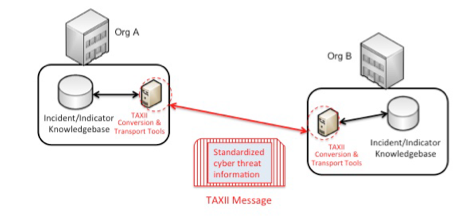
\includegraphics[scale=0.80]{./images/TAXIIArchitecture1.png}
    \caption{Arquitectura de TAXII \protect\cite{b1}}
    \label{fig.diagramabloques}
\end{figure}

TAXII utiliza protocolos y especificaciones existentes siempre que 
es posible, de esta forma se integra con mecanismos de intercambio de 
información para reducir los costos de implementación y permitir la adopción 
rápida por parte de organizaciones ya establecidas y que se encuentran 
intercambiando información.\\

Las motivaciones para tener una mejor solución que permita intercambiar 
información lleva a que en el diseño de TAXII se hayan planteado los siguientes 
objetivos:
 \begin{itemize}
   \item Permitir el intercambio seguro y rápido de información referente a 
   amenazas entre comunidades de defensores de seguridad.
   \item Lograr un estándar para permitir compartir indicadores entre organizaciones.
   \item Extender el intercambio de indicadores para permitir intercambios 
   seguros, robustos y de gran volumen que tengan una expresividad mayor a la 
   actual.
   \item Soportar un amplio número de casos de uso y prácticas comunes a las 
   comunidades.
   \item Tomar los estándares existentes que sean adecuados.
   \item Llegar a una adopción por parte de organizaciones internacionales de 
   estándares.
 \end{itemize}

Para automatizar el intercambio de información, es necesario especificar como 
ésta es compartida. Para lograr esto, TAXII define especificaciones técnicas y 
documentación de soporte. En particular, las especificaciones de TAXII definen 
un conjunto de capacidades necesarias para el transporte exitoso de mensajes. 
Los mensajes TAXII llevan datos de amenazas informáticas representados por medio de STIX. El conjunto completo de los mensajes incluyen mensajes con datos y 
de control.\\

\subsubsection{TAXII Toolkit}\ \\

Es provisto para soportar la adopción de TAXII y asistir en el desarrollo de 
capacidades compatibles. El \textit{toolkit} provee una colección de implementaciones de 
referencia, un conjunto de herramientas y una colección de librerías e 
interfaces.\\

TAXII está definido por múltiples especificaciones relacionadas. Esta sección 
describe las especificaciones definidas en TAXII.

\begin{itemize}
  \item \underline{Especificación de servicios}: Provee los requerimientos por los cuales se 
  definen los servicios e intercambios de TAXII. No provee detalles respecto al 
  formato de los datos o como los mensajes TAXII son transportados por la red. 
  Dichos detalles y requerimientos pueden ser encontrados en la especificación 
  de los protocolos de enlace y en la especificación de mensajes de enlace.
 \item \underline{Especificación de protocolos de enlace}: Define los requerimientos para 
 transportar mensajes TAXII por la red. Puede haber varias especificaciones 
 creadas para TAXII. Cada especificación define requerimientos para el 
 transporte de mensajes TAXII utilizando protocolos de red y se proveen 
 requerimientos respecto a como los servicios TAXII son soportados por los 
 protocolos de red.
 \item \underline{Especificación de mensajes de enlace}: Se definen requerimientos para 
 representar mensajes TAXII en un formato particular. Puede haber múltiples 
 especificaciones para dichos mensajes. Se provee información detallada sobre 
 como las especificaciones definidas en la especificación de servicios son 
 expresadas en los mensajes.
\end{itemize}

Para dar flexibilidad en el proceso evolutivo de TAXII, se han separado las 
especificaciones de servicios, de los protocolos de enlace y de los mensajes de 
enlace.
Debido a que las organizaciones generalmente tienen restricciones 
respecto a los protocolos que soportan, TAXII busca no ligarse a un único 
protocolo que excluya a una parte de la comunidad. Cuando se ve que la comunidad 
expresa interés en un nuevo protocolo o tipo de mensaje, TAXII puede dar soporte 
para ellos sin cambiar los componentes centrales.\\

Dos grupos que usen el mismo protocolo de red y formato de mensajes serán 
capaces de intercambios de información estructurada de forma automática. Las 
políticas de intercambio de los participantes pueden limitar estos intercambios 
si es necesario, pero el uso de servicios compatibles con TAXII asegura que se 
puede intercambiar cualquier información con los mecanismos definidos por TAXII. 
Los grupos que usen diferentes protocolos o formatos de mensajes no serán 
capaces de comunicarse directamente, pero como están utilizando mensajes y 
servicios en el núcleo de las comunicaciones de sus comunidades significa que es 
posible establecer caminos para que ocurra la interacción.

\subsubsection{Especificación de Servicios}\ \\

Esta especificación provee normativas respecto a los servicios, mensajes e 
intercambios de mensajes en TAXII. No provee detalles respecto a como los 
mensajes son transportados, dejando eso a la especificación de los protocolos de 
enlace. Se da información respecto a los datos presentes en los mensajes TAXII y 
no a como los mensajes son expresados.\\

Las unidades funcionales de TAXII representan conjuntos discretos de actividades 
requeridas para soportar TAXII. Una unidad funcional representa algún componente 
con un rol bien definido en TAXII.

\begin{itemize}
  \item \underline{TAXII Transfer Agent} (TTA): Es una unidad funcional conectada a la red 
  que envía o recibe mensajes TAXII. Una TTA interactúa con otras TTAs por medio 
  de la red y maneja los requerimientos de una o más de las especificaciones de 
  los protocolos de enlace. Una TTA provee un mensaje TAXII a un \textit{TAXII Message 
  Handler} permitiendo que éste último sea independiente del protocolo de red 
  utilizado. De la misma forma, el TTA puede ser independiente del contenido de 
  los mensajes TAXII, dejando el manejo de la información al \textit{TAXII Message 
  Handler}.
  \item \underline{TAXII Messsage Handler} (TMH): Es una unidad funcional que produce y 
  consume mensajes TAXII. EL TMH es responsable de parsear y construir mensajes 
  con el formato especificado en uno o más TAXII \textit{Message Binding Specifications}. 
  Un TMH interactúa con un TTA, el cual maneja los detalles necesarios para 
  transmitir mensajes por la red. El Backend TAXII interactúa con el TMH para 
  convertir su contenido en mensajes TAXII y llevar a cabo actividades basadas 
  en los mensajes TAXII que son recibidos por el TMH.
  \item \underline{Backend TAXII}: Cubre todas las unidades funcionales distintas al TTA y 
  al TMH. Las especificaciones de TAXII no proveen requerimientos sobre como son 
  implementadas las capacidades en un backend más allá de como debe interactuar 
  con el TMH. Las organizaciones o implementadores pueden decidir que 
  capacidades implementar según los servicios TAXII que deseen soportar o según 
  como quieran dar ese soporte.
  \item \underline{Arquitectura TAXII}: Cubre los aspectos de las unidades funcionales de la 
  infraestructura de productor o consumidor que provee o utiliza servicios 
  TAXII. Una arquitectura TAXII incluye una TTA, un TMH y un backend TAXII.
  \end{itemize}

Lo expresado anteriormente se puede ver en la figura \ref{fig.unidades_funcionales}.

\begin{figure}[ht!]
  \centering
    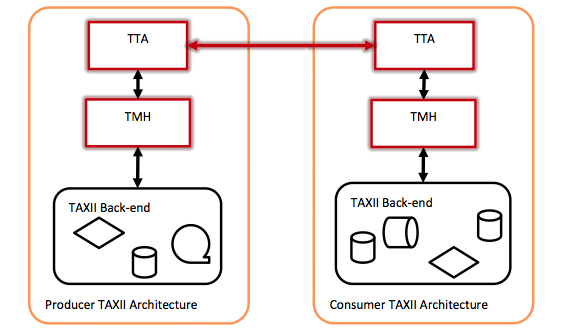
\includegraphics[width=150mm]{./images/TAXIIArchitecture.png}
    \caption{Unidades funcionales de TAXII \protect\cite{b1}}
    \label{fig.unidades_funcionales}
\end{figure}

\newpage
\subsubsection{Capacidades}\ \\

TAXII provee capacidades específicas para aquellos que desean compartir 
información de amenazas cibernéticas. Las capacidades TAXII son el nivel más 
alto en el cual se pueden expresar las acciones de TAXII. Hay tres capacidades 
que soporta la actual versión de TAXII, estas son: \textit{push messaging}, \textit{pull 
messaging} y \textit{discovery}.\\

En \textit{\textbf{push messaging}} la información puede ser enviada de un productor a un 
consumidor. Esto puede reflejar una relación pre-existente entre el productor y 
el consumidor en la que el consumidor ha pedido que se le envíen datos desde el 
productor. También puede usarse en caso de que el consumidor desee aceptar 
contribuciones de cualquier productor, y estos le envíen datos en cualquier 
momento.\\

\textit{\textbf{Pull messaging}} permite a un consumidor requerir información de un productor. 
Esto no solo le permite al consumidor el control sobre el momento en el que 
recibe los datos sino que también le permite hacerlo sin tener que aceptar 
conexiones entrantes. Así como en \textit{push messaging}, el productor y consumidor 
pueden tener acuerdos pre-existentes para que el consumidor tenga acceso a los 
datos del productor. De forma alternativa, un productor puede hacer su 
información pública de forma que cualquier consumidor pueda obtenerla. La 
versión actual de \textit{pull messaging} limita a los consumidores a hacer pedidos por 
medio de las organizaciones productoras de los datos en lugar de por los datos 
en si. Toda la información provista por un productor debe estar organizada en 
grupos llamados "TAXII Data Feeds". Cada elemento en un TAXII data feed es 
etiquetado utilizando \textit{timestamps}. El productor tiene total dominio sobre como el 
contenido se mapea en TAXII data feeds y en el significado de los \textit{timestamps}. La 
capacidad de \textit{pull messaging} está atada a entender el contenido del productor.\\

Para facilitar las comunicaciones automatizadas, TAXII soporta capacidades para 
descubrir los servicios específicos que ofrece un servidor o grupo de 
servidores, así como los protocolos o mensajes que este servidor ofrece. Esto no 
quita la necesidad de que personas estén involucradas para establecer acuerdos de 
cooperación lo cual esta por fuera del objetivo de TAXII. Sin embargo, permite 
el intercambio de información respecto a las capacidades que un productor 
soporta y cuales son los mecanismos que utiliza para hacerlo.

\subsubsection{Servicios TAXII}\ \\

Los servicios TAXII representan un conjunto de mecanismos necesarios para 
soportar capacidades TAXII. Una implementación TAXII pudiera implementar alguno, 
todos o incluso ninguno de los servicios definidos.
TAXII define los siguientes servicios:
\begin{itemize}
  \item \underline{Discovery Service}: Es utilizado para recibir y responder a 
  mensajes que requieren información sobre los servicios ofrecidos.
  \item \underline{Feed Managment Service}: Es utilizado para recibir o responder a mensajes 
  utilizados para el manejo de subscripciones a TAXII Data Feed.
  \item \underline{Inbox Service}: Es utilizado para recibir información de amenazas 
  cibernéticas por medio de intercambios iniciados por el productor en intervalos 
  dictados por este.
  \item \underline{Poll Service}: Es utilizado para recibir y responder a mensajes de pedido 
  a el TAXII Data Feed iniciados por el consumidor.
\end{itemize}

A continuación se describen los distintos servicios.

\paragraph{Discovery Service}\ \\

Es un mecanismo para comunicar información referente al uso de servicios TAXII y 
a su disponibilidad. Para un pedido al servicio, se retorna una lista de los 
servicios TAXII y como estos pueden ser invocados. Un solo servicio de 
descubrimiento puede reportar servicios TAXII en diferentes equipos finales o 
incluso en múltiples organizaciones, los propietarios del servicio pueden 
definir su alcance a gusto. Un servicio de descubrimiento puede utilizar 
varios factores para determinar cuales servicios revelar ante una petición, 
incluyendo, pero no limitado a la entidad del cliente TAXII.
El servicio de descubrimiento debe soportar "Discovery Message Exchange".

\paragraph{Feed Managment Service}\ \\

Es el mecanismo con el cual un consumidor pide información referente a TAXII 
Data Feeds, pidiendo subscripciones a estos, o modificando las existentes. Este 
servicio facilita el intercambio de mensajes para manejar las subscripciones. 
No se entrega contenido de los TAXII Data Feed, en su lugar se envía 
contenido del TAXII Data Feed al servicio de Inbox de un consumidor en intercambios 
iniciados por un productor o en respuesta directa a un pedido del consumidor al 
servicio de poll.
Dicho servicio debe implementar soporte para \textit{subscription managment exchange} y podría implementar soporte de \textit{feed information exchange}.

\paragraph{Inbox service}\ \\
Este servicio es el mecanismo con el cual un consumidor acepta los mensajes en 
un intercambio iniciado por el productor. Un consumidor puede implementarlo 
para recibir datos del TAXII Data Feed.
El servicio de inbox debe implementar soporte para \textit{Data Push Exchange}.

\paragraph{Poll service}\ \\
Es provisto por un productor para permitir pedidos al TAXII Data Feed iniciados 
por  el consumidor. Un consumidor contacta a este servicio explícitamente 
pidiendo el contenido del TAXII Data Feed. Los productores podrían ofrecer Data 
Feeds combinando envíos al Inbox service del consumidor o por medio de pedidos 
al servicio de poll del productor.
Una implementación de este servicio debe dar soporte a \textit{Data Poll Exchange}.

\subsubsection{Intercambio de mensajes TAXII}\ \\

Esta sección describe los mensajes intercambiados que son necesarios para soportar 
los servicios definidos antes. Estos intercambios solo consideran mensajes 
TAXII y son independientes a los protocolos sobre los cuales viajan los mensajes.
 En particular, esos protocolos podrían requerir intercambios de red 
adicionales antes de transmitir mensajes TAXII o romper un mensaje TAXII en 
múltiples mensajes del protocolo subyacente que son transmitidos 
independientemente.

\paragraph{Data Push Exchange}\ \\
En este intercambio, un mensaje STIX es transmitido desde un cliente a un 
servidor inbox que está esperando. El mensaje STIX puede ser solicitado o no 
solicitado. El servidor inbox puede ser capaz de filtrar mensajes según la 
autenticidad del emisor.

\paragraph{Discovery Exchange}\ \\

Un cliente TAXII pide información sobre el servicio TAXII ofrecido por un 
productor. El discovery server del productor responde con una lista de 
servicios. 

El cliente TAXII envía un pedido de descubrimiento al servidor. El Backend TAXII podría utilizar esta 
información junto a su propia política de control de acceso  para crear una 
lista de servicios a ser retornada. Estos son empaquetados en una 
respuesta de discovery la cual es enviada al cliente TAXII. El 
cliente TAXII recibe esa respuesta y la pasa la información del servicio a su 
propio BackEnd para ser procesado.

\paragraph{Feed Information Exchange}\ \\

En este intercambio un cliente TAXII pide información sobre fuentes de datos disponibles en 
un Feed Server. El servidor responde con una lista de fuentes de datos 
de las que dispone. Dicha respuesta es realizada por el backend y en ella se pueden considerar decisiones de control de acceso.\\

\paragraph{Subscription Managment Exchange}\ \\

En este un cliente intenta establecer, borrar, pausar, resumir o modificar una 
subscripción a un TAXII Data Feed conocido enviando un mensaje subscription 
managment request al servidor. El servidor pasa la request al Backend TAXII el 
cual determina la respuesta, la cual es luego enviada al cliente.
El backend TAXII puede usar dicha información junto con sus 
políticas de control de acceso y las funcionalidades que posea para determinar 
si la acción está permitida o no.

\paragraph{Feed Poll Exchange}

Es utilizado por un consumidor para pedir contenido de un productor de datos. El TAXII Data Feed content es enviado al consumidor en el mismo intercambio.
El cliente consumidor inicia el backend TAXII y evalua el pedido de información para determinar la respuesta. La respuesta retorna mensajes STIX con el contenido que pidió el cliente.
 
%\subsubsection{Modelos}
%\label{anexo.modelos}
%\subsubsection{Comunidades}
Actualmente el número de organizaciones que buscan compartir información de
amenazas es creciente. Esto lleva a que el número y tipo de comunidades que busca
hacerlo también se incremente. En la actualidad se identifican tres tipos de comunidades:
\begin{itemize}
  \item Pares
  \item Comerciales
  \item Gubernamentales
\end{itemize}

Para que se pueda compartir información entre dichas organizaciones es necesario
cierto nivel de confianza dado que compartir información sensible podría exponer 
a las organizaciones a daños en su reputación, demandas o advertir a un 
atacante de la investigación que se lleva a cabo haciendo que el trabajo 
realizado haya sido inútil. Se deben definir medidas para la protección de los 
datos como restricciones en su manejo, sanitización y el establecimiento de 
confianza entre las dos organizaciones. Lo mencionado anteriormente es 
particularmente importante cuando las organizaciones forman parte de varias 
comunidades que intercambian información, se encuentran casos en los que datos 
compartidos con una organización no deberían ser compartidos con otra.\\

Las comunidades entre \textbf{pares} son las más comunes, estas organizaciones o 
individuos tienen el propósito común de mejorar las defensas colectivas contra 
adversarios que tienen en común. La información compartida por dichas 
organizaciones es más especifica que la provista por organizaciones comerciales.\\

Las comunidades \textbf{comerciales} son anónimas y los miembros poseen algún tipo de 
acuerdo común, por ejemplo el pago de cuotas para pertenecer a la comunidad. 
La organización comercial maneja la información de forma centralizada y la 
distribuye entre los miembros de la organización. El acceso a la información por 
parte de los socios es rápido teniendo la posibilidad de que dicha información 
sea más amplia que la compartida por pares y que además no siempre sea aplicable a las 
necesidades de la organización.\\

Las comunidades \textbf{gubernamentales} son establecidas y manejadas por el gobierno, 
son voluntarias u obligatorias e incluyen participantes tanto del gobierno como 
de la industria privada. En ellas el gobierno controla la información y la 
distribución de esta. Así como en las comunidades comerciales, la información y 
los participantes son altamente confidenciales.\\

\subsubsection{Modelos}

Se pueden identificar tres modelos para el intercambio de información entre 
organizaciones:
\begin{itemize}
  \item Hub and Spoke
  \item Peer to peer
  \item Source/subscriber
\end{itemize}

En el método \textbf{hub and spoke}, la entidad hub controla la recepción y diseminación 
de los datos, además se encarga de mantener anónimos y proveer un análisis 
adicional de los datos recolectados para luego diseminarlos entre los 
participantes. Este modelo es comúnmente visto en comunidades de gobierno o comerciales.\\

En el modelo \textbf{peer to peer}, los participantes intercambian y reciben información 
directamente de los otros participantes. La información es compartida entre 
todos los miembros de la comunidad por igual y la fuente está claramente 
identificada.\\

\textbf{Source/subscriber} es utilizado por las 
comunidades comerciales que proveen de información. El proveedor de información 
envía regularmente información a todos los subscriptores y estos podrían 
eventualmente enviarle información a la fuente. Generalmente, la información se 
codifica de una manera propietaria y puede faltar información esencial sobre 
algunos intentos de irrupción. Presenta la ventaja de que se tiene acceso rápido 
a un conjunto de datos amplio y es útil para organizaciones con recursos 
limitados.\\

\subsubsection{Implementación de Modelos en TAXII}

A continuación se muestra como los servicios TAXII pueden ser utilizados para la 
implementación de los modelos para el intercambio de información.

\paragraph{Source/Suscriber}\ \\

En este modelo una entidad es la fuente de información y algunos subscriptores 
tienen acuerdos con dicha entidad para recibir información periódicamente. Se 
busca que los subscriptores no se conozcan entre si, para ello la entidad fuente 
realiza acuerdos con cada uno de ellos. En este modelo, la fuente es 
un productor TAXII mientras que los subscriptores son consumidores.\\

TAXII soporta este tipo de modelo para el intercambio con el uso de los servicios de 
Discovery, Feed Management, Inbox y Poll. Una organización que desee 
subscribirse al TAXII Data Feed de la fuente necesita conocer los servicios 
TAXII que la fuente ofrece y como contactar con ellos. Si bien esto podría ser 
realizado por una mecanismo fuera de banda (e.g. publicando la información en otro medio)
también podría ser logrado contactando al Discovery Service de la fuente. Desde 
este punto, el subscriptor podría contactar al servicio de Feed Managment 
identificado para aprender que fuentes ofrece el productor y que restricciones 
podría tener su acceso.\\

Si el contenido del TAXII Data Feed es restringido solo a algunas entidades 
autorizadas y el productor ha determinado que el subscriptor tiene permitido 
recibir el contenido, la fuente y el subscriptor necesitan acordar en como el 
subscriptor se autenticara. Dependiendo en el protocolo que soporta la fuente, 
esto se puede realizar por medio de una contraseña, un certificado u otro método. 
Si el contenido de un TAXII Data Feed es abierto y no requiere 
autenticación, éste paso es innecesario cuando se establecen las subscripciones 
al TAXII Data Feed.\\

Luego de la autenticación,el subscriptor puede contactar al Feed Managment Service del 
productor y pedir subscripciones a sus fuentes. La entidad fuente puede 
comparar dichos pedidos con su propio entendimiento de lo que el subscriptor 
puede recibir y permitir o denegar dichos pedidos según corresponda. La fuente 
puede enviar contenido al subscriptor al Inbox Service de éste en el intervalo 
apropiado. Alternativamente, el subscriptor podría contactar al Poll service de 
la fuente para descargar el contenido deseado.\\

\begin{figure}[ht!]
 
  \centering
  	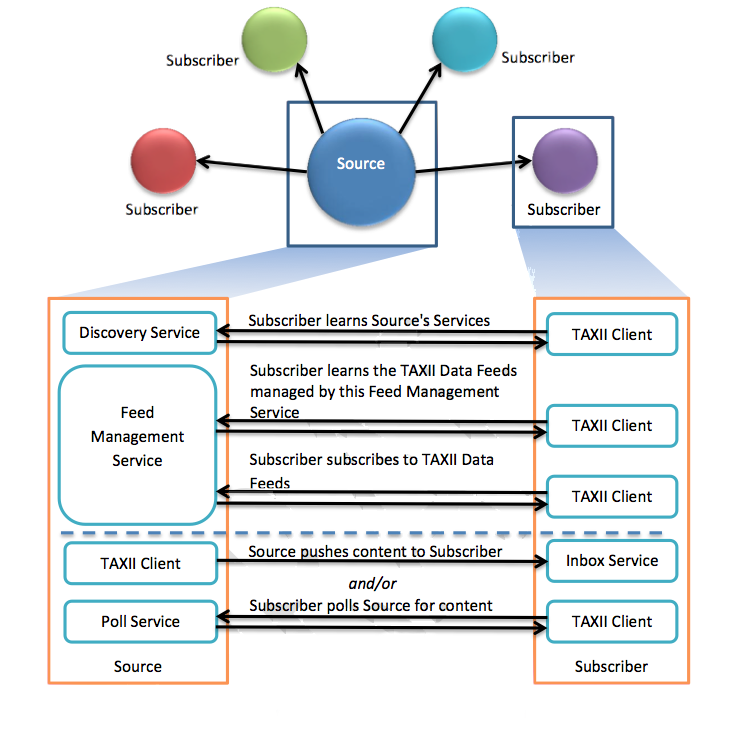
\includegraphics[width=150mm]{./images/SourceSuscriberModel.png}
    \caption{Flujo de información en modelo Source/Subscriber \protect\cite{b1}}
    \label{fig.sourcesuscribermodel}
\end{figure}

La figura \ref{fig.sourcesuscribermodel} muestra como el modelo Source/Subscriber puede ser soportado por los 
servicios TAXII. También se ven los mensajes TAXII intercambiados entre la
fuente y el subscriptor. Con los intercambios que están por encima de la línea 
punteada se establece la subscripción. Los intercambios pueden ser realizados 
repetidamente sin la necesidad de realizar el proceso de subscripción 
nuevamente.

\newpage

\paragraph{Peer-to-peer}\ \\ 

En un modelo Peer-to-peer, los pares de organizaciones entran en un acuerdo 
mutuo para compartir información entre si. En este modelo, cada Peer puede 
operar como productor y consumidor. Los socios en este intercambio podrían 
establecer fuentes utilizando un procedimiento similar al establecido en el 
modelo Source/Subscriber. Alternativamente, podrían acordar subir o descargar 
contenido sin ninguna subscripción formal. No tener una subscripción formal 
permite a un Peer albergar un Inbox Service sin necesidad de un Feed 
Managment Service.\\

El modelo Peer-to-Peer tiene dos variantes: acuerdos para el intercambio entre 
comunidades y acuerdos para el intercambio ad-hoc. En el primero la comunidad 
constituye acuerdos entre pares en los que todos los miembros acuerdan una única 
política la cual será respetada por todos. A diferencia de los otros dos 
modelos que tienen un punto central desde el cual la información es diseminada, 
todo el intercambio ocurre puntualmente entre dos pares. Si los pares A y B 
desean recibir información del peer C directamente, ambos necesitaran 
establecer un acuerdo apropiado con el peer C para que éste les envíe la 
información que desean.\\

Alternativamente, el intercambio entre pares puede ser realizado de forma 
individual con intercambios ad-hoc. Esto podría ocurrir si dos compañías hacen 
acuerdos individuales para compartir entre ellas. En este caso, los acuerdos 
sobre que compartir son específicos para las partes. Una sola entidad podría 
participar en ambas variantes, perteneciendo a una o mas comunidades en las 
cuales los miembros comparten entre si siguiendo un acuerdo común entre los 
miembros y a su vez negocian acuerdos individuales con otras entidades. Alguna 
información recibida por medio de un acuerdo no siempre debería ser compartida 
con otros pares que no son parte del acuerdo. De esta forma un participante 
debería hacer un seguimiento de quien fue el proveedor de la información 
recibida, como se realiza ese seguimiento está por fuera de la especificación de 
TAXII.\\

\begin{figure}[ht!]
  \centering
  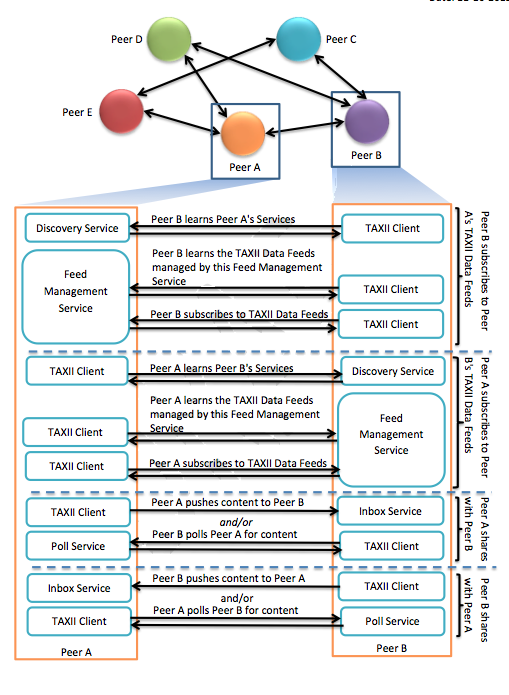
\includegraphics[scale=0.55]{./images/PeerToPeerModel.png}
    \caption{Flujo de información en modelo Peer to Peer \protect\cite{b1}}
  \label{fig.peertopeermodel}
\end{figure}

La figura \ref{fig.peertopeermodel} muestra como el modelo Peer to peer puede ser realizado por 
medio de los servicios TAXII. En este diagrama se ve que dos pares se contactan 
para pedir subscripciones para obtener información. Se asume que ambos pares 
tienen un Feed Managment Service que es utilizado para manejar todos los 
pedidos de subscripción.
\newpage

\paragraph{Hub and Spoke}\ \\

En un modelo Hub and Spoke, la entidad Hub es un consumidor de 
información que le proveen las entidades Spoke, pero a su vez se comporta como
un productor que brinda información a entidades 
Spoke. Una entidad Spoke podría ser un productor, dando información al Hub, un 
consumidor que reciba actualizaciones del Hub o ambas. El Hub puede utilizar un 
Inbox Service para recibir información de cualquiera que desee enviar 
información de forma voluntaria y/o podría requerir información de ciertas 
fuentes para guardar la información en una única ubicación. Desde este punto, el 
Hub puede funcionar como una entidad Source del modelo Source/Subscriber 
mientras que los Spoke serían Subscribers de dicho modelo. El Hub puede adoptar 
cualquier política respecto de la información que recibe, desde pasar toda la 
información automáticamente a solo pasar información de socios reconocidos, o 
realizar ediciones y análisis antes de reenviar la información.

\begin{figure}[ht!]
  \centering
    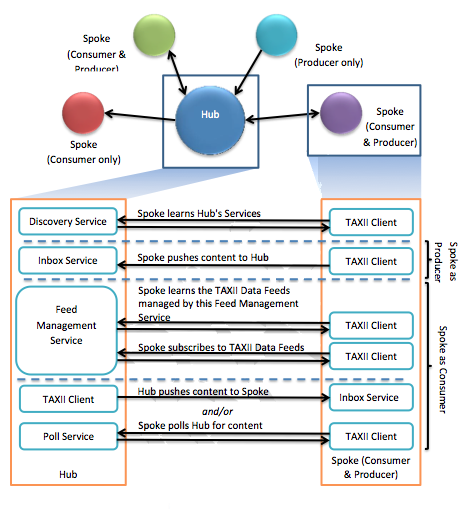
\includegraphics[scale=0.75]{./images/HubAndSpokeModel.png}
    \caption{Flujo de información en modelo Hub and Spoke \protect\cite{b1}}
    \label{fig.hubandspokemodel}
\end{figure}

La figura \ref{fig.hubandspokemodel} muestra como se puede implementar el modelo Hub and Spoke 
utilizando los servicios provistos por TAXII. En este modelo algunas entidades 
Spoke podrían ser consumidores, otras productores y en algunos casos ambas. El 
diagrama muestra los intercambios que podrían ser utilizados por el Spoke que 
actúa como productor y consumidor. Si este desea actuar de una sola forma solo 
los intercambios necesarios serían relevantes. Independientemente del rol que 
tome el Spoke, es necesario que éste conozca los servicios relevantes en el Hub. 
Esto se realiza utilizando el Discovery Service provisto por el Hub, de todas 
formas esto podría realizarse con mecanismos fuera de banda.



 

\section{Implementación}
\subsection{Servicios TAXII Implementados}
	
	\begin{center}
		\begin{tabular}{|l|}
			\hline
			def inbox\service(request, inbox\name): \\
			"""Handles TAXII Inbox Service requests.""" \\ \\
			
			def poll\service(request):\ \\
			"""Handles TAXII Poll Service requests.""" \\ \\
			
			def feed\managment\service(request): \\
			"""Handles TAXII Feed Managment Service requests.""" \\ \\
			
			def subscription\service(request):\ \\
			"""Handles TAXII Subscription Service requests.""" \\
			\hline
		\end{tabular}
	\end{center}\ \\

\subsection{API REST implementada}

	\begin{center}
		\begin{tabular}{|l|}
			\hline
			class UserViewSet(viewsets.ModelViewSet):\\
			\#Gets, lists, creates or updates users.\\ \\
			
			class ProtocolBindingIdViewSet(viewsets.ModelViewSet):\\
			\#Gets, lists, creates or updates ProtocolBindingIds\\ \\
			
			class ContentBindingIdViewSet(viewsets.ModelViewSet):\\
			\#Gets, lists, creates or updates ContentBindingIds\\ \\
			
			class MessageBindingIdViewSet(viewsets.ModelViewSet):\\
			\#Gets, lists, creates or updates MessageBindingIds\\ \\
			
			class DataFeedPushMethodViewSet(viewsets.ModelViewSet):\\
			\#Gets, lists, creates or updates DataFeedPushMethods\\ \\
			
			class DataFeedPollInformationViewSet(viewsets.ModelViewSet):\\
			\#Gets, lists, creates or updates DataFeedPollInformations\\ \\
			
			class RemoteDataFeedPollInformationViewSet(viewsets.ModelViewSet):\\
			\#Gets, lists, creates or updates RemoteDataFeedPollInformations\\ \\
			
			class DataFeedSubscriptionMethodViewSet(viewsets.ModelViewSet):\\
			\#Gets, lists, creates or updates DataFeedSubscriptionMethods\\ \\
			
			class ContentBlockViewSet(viewsets.ModelViewSet):\\
			\#Gets, lists, creates or updates ContentBlocks\\ \\
			
			class DataFeedViewSet(viewsets.ModelViewSet):\\
			\#Gets, lists, creates or updates DataFeeds\\ \\
			
			class RemoteDataFeedViewSet(viewsets.ModelViewSet):\\
			\#Gets, lists, creates or updates RemoteDataFeeds\\ \\
			
			class DataFeedSubscriptionViewSet(viewsets.ModelViewSet):\\
			\#Gets, lists, creates or updates SubscriptionFeeds\\
			
			\hline
		\end{tabular}
	\end{center}
	\newpage
	\begin{center}
		\begin{longtable}{|l|}
			\hline
			
			class InboxViewSet(viewsets.ModelViewSet):\\
			\#Gets, lists, creates or updates Inboxes\\ \\
			
			class RemoteInboxViewSet(viewsets.ModelViewSet):\\
			\#Gets, lists, creates or updates RemoteInboxes\\ \\
			
			class ContentBlockRTIRViewSet(viewsets.ModelViewSet):\\
			\#Gets, lists, creates or updates ContentBlockRTIRs\\ \\
			
			class TAXIIServicesViewSet(viewsets.ModelViewSet):\\
			\#Gets, lists, creates or updates TAXIIServices\\ \\
			
			class FeedManagmentServicesViewSet(viewsets.ModelViewSet):\\
			\#Gets, lists, creates or updates FeedManagementServices\\ \\
			
			
			def get\remote\data\feeds(request):\\
			\#Given the id of a TAXII Service we make a FeedInformation request to\\ that service address.\\
			\#The response is a list of the feed names of the TAXII client and\\ a list of all protocol bindings,\\ content binding and message binding.\\ \\
			
			def register\remote\data\feeds(request):\\
			\#Given the id of a TAXII service we get the data feeds of the TAXII Client and\\ copy them to the current system.\\ \\
			
			def create\information(request):\\
			\#When in GET method return all the Content Blocks.\\
			\#When in POST method, given a content binding id, a title, description and content\\ we create a Content Block.\\ \\
			
			def send\information\to\inbox(request):\\
			\#Given the id of a DataFeed Subscription we get the Data Feeds and send it to\\ send it to the inbox service of the organization of the subscription service.\\ \\
			
			def poll\information(request):\\
			\#Given the id of a remote data feed,\\ we get the poll service instances and for each make a poll request.\\ \\
			
			def get\data\feed\subscriptions(request):\\
			\#We get all the date feed subsctiptions and\\ return the id, adress and data feed name of each.\\ \\
			
			def subscription\to\data\feed(request):\\
			\#Given the id of a TAXII Service and the id of a Data Feed and\\ the service id we make a Manage Feed Subscription request for that Data Feed.\\		
			
			\hline
		\end{longtable}
	\end{center}
	\newpage

\subsection{Entidades desarrolladas utilizadas}
	
	\begin{center}
		\begin{longtable}{|l|}
			\hline

	class ProtocolBindingId():\\
	    """\\
	    Represents a protocol binding id, used to establish the exchange protocol\\
	    supported by a TAXII implementation.\\
	    Ex:\\
	    HTTP protocol binding id : "urn:taxii.mitre.org:protocol:http:1.0"\\
	    HTTPS protocol binding id : "urn:taxii.mitre.org:protocol:https:1.0"\\
	    """\\
	    title = CharField(blank=True)\\
	    description = TextField(blank=True)\\
	    bindingid = CharField(maxlength=MAXIDLEN)\\
	    datecreated = DateTimeField(autonowadd=True)\\
	    dateupdated = DateTimeField(autonow=True)\\
	\\
	class ContentBindingId():\\
	    """\\
	    Represents a content binding id, used to establish the supported content\\
	    types for a given TAXII exchange (e.g., Poll, Inbox, etc.).\\
	    Ex:\\
	    STIX v1.0 content binding id : "urn:stix.mitre.org:xml:1.0"\\
	    """\\
	    title = CharField(blank=True)\\
	    description = TextField(blank=True)\\
	    bindingid = CharField(maxlength=MAXIDLEN)\\
	    datecreated = DateTimeField(autonowadd=True)\\
	    dateupdated = DateTimeField(autonow=True)\\
	\\
	class MessageBindingId():\\
	    """\\
	    Represents a message binding id, used to establish the supported syntax\\
	    for a given TAXII exchange, "e.g., XML".\\
	    Ex:\\
	    XML message binding id : "urn:taxii.mitre.org:message:xml:1.0"\\
	    """\\
	    title = CharField(blank=True)\\
	    description = TextField(blank=True)\\
	    bindingid = CharField(maxlength=MAXIDLEN)\\
	    datecreated = DateTimeField(autonowadd=True)\\
	    dateupdated = DateTimeField(autonow=True)\\
	\\
	class DataFeedPushMethod():\\
	    """\\
	    Used to establish the protocols that can be used to push content via\\
	    a subscription. This appears in a Feed Information Response message,\\
	    as defined by the TAXII Services Specification.\\
	    """\\
	    title = CharField(blank=True)\\
	    description = TextField(blank=True)\\
	    protocolbinding = ForeignKey(ProtocolBindingId)\\
	    messagebinding = ForeignKey(MessageBindingId)\\
	    datecreated = DateTimeField(autonowadd=True)\\
	    dateupdated = DateTimeField(autonow=True)\\
	\\
	class DataFeedPollInformation():\\
	    """\\
	    Used to establish the supported protocols and address of a Data Feed.\\
	    This appears in a Feed Information Response message, as defined by the\\
	    TAXII Services Specification.\\
	    """\\
	    title = CharField(blank=True)\\
	    description = TextField(blank=True)\\
	    address = URLField()\\
	    protocolbinding = ForeignKey(ProtocolBindingId)\\
	    messagebindings = ManyToManyField(MessageBindingId)\\
	    datecreated = DateTimeField(autonowadd=True)\\
	    dateupdated = DateTimeField(autonow=True)\\
	\\
	class DataFeedSubscriptionMethod():\\
	    """\\
	    Used to identify the protocol and address of the TAXII daemon hosting\\
	    the Feed Management Service that can process subscriptions for a TAXII\\
	    Data Feed. This appears in a Feed Information Response message, as defined\\
	    by the TAXII Services Specification.\\
	    """\\
	    title = CharField(blank=True)\\
	    description = TextField(blank=True)\\
	    address = URLField()\\
	    protocolbinding = ForeignKey(ProtocolBindingId)\\
	    messagebindings = ManyToManyField(MessageBindingId)\\
	    datecreated = DateTimeField(autonowadd=True)\\
	    dateupdated = DateTimeField(autonow=True)\\
	\\
	class ContentBlock():\\
	    """Represents the content block of a TAXII Poll Response or Inbox message."""\\
	    title = CharField(blank=True) # not required by TAXII\\
	    description = TextField(blank=True) # not required by TAXII\\
	    timestamplabel = DateTimeField(default=lambda:datetime.datetime.now(tzutc()))\\
	    submittedby = ForeignKey(User, blank=True, null=True)\\
	    messageid = CharField(blank=True)\\
	    contentbinding = ForeignKey(ContentBindingId)\\
	    content = TextField()\\
	    padding = TextField(blank=True)\\
	    datecreated = DateTimeField(autonowadd=True)\\
	    dateupdated = DateTimeField(autonow=True)\\
	\\
	class DataFeed():\\
	    """Represents a TAXII Data Feed"""\\
	    name = CharField()\\
	    description = TextField(blank=True)\\
	    users = ManyToManyField(User, blank=True, null=True)\\
	    supportedcontentbindings = ManyToManyField(ContentBindingId)\\
	    pushmethods = ManyToManyField(DataFeedPushMethod)\\
	    pollserviceinstances = ManyToManyField(DataFeedPollInformation)\\
	    subscriptionmethods = ManyToManyField(DataFeedSubscriptionMethod, blank=True, null=True)\\
	    contentblocks = ManyToManyField(ContentBlock, blank=True, null=True)\\
	    datecreated = DateTimeField(autonowadd=True)\\
	    dateupdated = DateTimeField(autonow=True)\\
	\\
	class DataFeedSubscription():\\
	    """Represents a Data Feed Subscription. This is not used by TAXII at the moment."""\\
	    subscriptionid = CharField(unique=True) # uri formatted subscription id\\
	    user = ForeignKey(User)\\
	    datafeed = ForeignKey(DataFeed)\\
	    datafeedmethod = ForeignKey(DataFeedSubscriptionMethod)\\
	    active = BooleanField(default=True)\\
	    expires = DateTimeField()\\
	    datecreated = DateTimeField(autonowadd=True)\\
	    dateupdated = DateTimeField(autonow=True)\\
	\\
	class Inbox():\\
	    """\\
	    Characterizes a TAXII Inbox. Inboxes are the mechanism by which TAXII consumers\\
	    receive data from TAXII publishers. This Inbox implementation allows an Inbox\\
	    to be "bound" to zero or more Data Feeds, meaning that data received by an Inbox\\
	    can populate Data Feeds if a user configures it as such.\\
	    """\\
	    name = CharField(unique=True)\\
	    description = TextField(blank=True)\\
	    supportedcontentbindings = ManyToManyField(ContentBindingId)\\
	    supportedmessagebindings = ManyToManyField(MessageBindingId)\\
	    contentblocks = ManyToManyField(ContentBlock, blank=True, null=True)\\
	    supportedprotocolbinding = ForeignKey(ProtocolBindingId)\\
	    datafeeds = ManyToManyField(DataFeed, blank=True, null=True)\\
	    users = ManyToManyField(User, blank=True, null=True)\\
	    datecreated = DateTimeField(autonowadd=True)\\
	    dateupdated = DateTimeField(autonow=True)\\
	\\
	class ContentBlockRTIR():\\
	    """Represents the nexus between the RTIR ticket and the content block."""\\
	    rtirid = IntegerField(unique=True)\\
	    contentblock = ForeignKey(ContentBlock)\\
	\\
	class RemoteDataFeedPollInformation():\\
	    """Represents DataFeed Poll Information of remote TAXII clients """\\
	    title = CharField(blank=True)\\
	    description = TextField(blank=True)\\
	    address = URLField()\\
	    protocolbinding = ForeignKey(ProtocolBindingId)\\
	    messagebindings = ManyToManyField(MessageBindingId)\\
	    datecreated = DateTimeField(autonowadd=True)\\
	    dateupdated = DateTimeField(autonow=True)\\
	\\
	class RemoteDataFeed():\\
	    """Represents DataFeeds of remote TAXII clients """\\
	    name = CharField(maxlength=MAXTITLELEN)\\
	    description = TextField(blank=True)\\
	    supportedcontentbindings = ManyToManyField(ContentBindingId)\\
	    pushmethods = ManyToManyField(DataFeedPushMethod)\\
	    pollserviceinstances = ManyToManyField(RemoteDataFeedPollInformation, null=True)\\
	    subscriptionmethods = ManyToManyField(DataFeedSubscriptionMethod, blank=True, null=True)\\
	    contentblocks = ManyToManyField(ContentBlock, blank=True, null=True)\\
	    datecreated = DateTimeField(autonowadd=True)\\
	    dateupdated = DateTimeField(autonow=True)\\
	\\
	class RemoteInbox():\\
	    """Represents Inboxes of remote TAXII clients """\\
	    name = CharField(unique=True) # this will become part of the URL where it can be accessed at\\
	    description = TextField(blank=True)\\
	    supportedcontentbindings = ManyToManyField(ContentBindingId)\\
	    supportedmessagebindings = ManyToManyField(MessageBindingId)\\
	    supportedprotocolbinding = ForeignKey(ProtocolBindingId)\\
	    datafeed = ForeignKey(DataFeed, blank=True)\\
	    address = URLField()\\
	    datecreated = DateTimeField(autonowadd=True)\\
	    dateupdated = DateTimeField(autonow=True)\\
	\\
	class TAXIIServices():\\
	    """Represents all TAXII Services available """\\
	    name = CharField(unique=True)\\
	    description = TextField(blank=True)\\
	    inbox = URLField()\\
	    poll = URLField()\\
	    feedmanagment = URLField()\\
	    subscription = URLField()\\
\\

			
			\hline
		\end{longtable}
	\end{center}
	
\subsection{Cyber Obsevables utilizados en el caso de estudio}

	\lstset{
		 breaklines=true
	}
    \lstinputlisting{cybox/CybOX_Artifact_Instance.xml}
	\lstinputlisting{cybox/CybOX_Artifact_Pattern.xml}
	\lstinputlisting{cybox/CybOX_CreateFile_Action.xml}
	\lstinputlisting{cybox/CybOX_Domain_Instance.xml}
	\lstinputlisting{cybox/CybOX_Domain_Pattern.xml}
	\lstinputlisting{cybox/CybOX_IPv4Address_Instance.xml}
	\lstinputlisting{cybox/CybOX_IPv4Address_Pattern.xml}
	\lstinputlisting{cybox/CybOX_IPv6Address_Instance.xml}
	\lstinputlisting{cybox/CybOX_IPv6Address_Pattern.xml}
	\lstinputlisting{cybox/CybOX_Iran-Oil_Dynamic.xml}
	\lstinputlisting{cybox/CybOX_Network_Connection_HTTP_Instance.xml}
	\lstinputlisting{cybox/CybOX_Network_Connection_HTTP_Pattern.xml}
	\lstinputlisting{cybox/CybOX_Network_Connection_Instance.xml}
	\lstinputlisting{cybox/CybOX_Network_Connection_Pattern.xml}
	\lstinputlisting{cybox/CybOX_PDF_File_Instance.xml}
	\lstinputlisting{cybox/CybOX_PDF_File_Pattern.xml}
	\lstinputlisting{cybox/CybOX_Simple_Email_Instance.xml}
	\lstinputlisting{cybox/CybOX_Simple_Email_Pattern.xml}
	\lstinputlisting{cybox/CybOX_Simple_File_Instance.xml}
	\lstinputlisting{cybox/CybOX_Simple_File_Pattern.xml}
	\lstinputlisting{cybox/CybOX_Simple_File_Pattern_Regex.xml}
	\lstinputlisting{cybox/CybOX_URL_Instance.xml}
	\lstinputlisting{cybox/CybOX_URL_Pattern.xml}
	\lstinputlisting{cybox/CybOX_X509_Certificate_Instance.xml}
	\lstinputlisting{cybox/CybOX_X509_Certificate_Pattern.xml}
